\documentclass[a4paper,openright,twoside,11pt]{report}

\usepackage[utf8]{inputenc}
\usepackage{lipsum}
\usepackage{graphicx}
\usepackage{url}
\usepackage[Algoritmo]{algorithm}
\usepackage{algorithmicx}
\usepackage{algpseudocode}
\usepackage{titlesec}
\usepackage{indentfirst}
\usepackage{subcaption}
\usepackage{amsmath}
\usepackage{listings}
\usepackage{xcolor}
\usepackage{fancyhdr} % For custom headers and footers

\setlength{\textheight}{24.00cm}
\setlength{\textwidth}{15.50cm}
\setlength{\topmargin}{0.35cm}
\setlength{\headheight}{0cm}
\setlength{\headsep}{0cm}
\setlength{\oddsidemargin}{0.25cm}
\setlength{\evensidemargin}{0.25cm}

\titleformat{\section}[block]{\normalfont\Large\bfseries}{\thesection}{1em}{}
\titlespacing*{\section}{0pt}{1cm}{0.5cm}

\titleformat{\subsection}[block]{\normalfont\large\bfseries}{\thesubsection}{1em}{}
\titlespacing*{\subsection}{0pt}{0.5cm}{0.4cm}

\titleformat{\subsubsection}[block]{\normalfont\normalsize\bfseries}{\thesubsubsection}{1em}{}
\titlespacing*{\subsubsection}{0pt}{1cm}{0.4cm}

% Title and Author

\title{
   \vspace{-50mm}
   \begin{minipage}[l]{\textwidth}
      \hspace{-5mm}\resizebox{75mm}{!}{
\includegraphics{./fcul_logo.png}}\\
   \end{minipage}\\[20mm]
   {\bf Privacy and Data Security Project}\\[5mm]
   {\bf First Delivery Report of Secure P2P Messaging App}\\[20mm]
}

\author{
    \begin{tabular}{ll}
        Henrique Alípio & 64452 \\
        Denis Ungureanu & 56307 \\ 
        Pedro Marques & 64857\\[50mm]
    \end{tabular}
}
\date{MEI \& MSI in Computer Science and Engineering}

\begin{document}

\maketitle
\newpage

% Introduction Section
\subsection*{Introduction}

The programming language used for this project is Java, with Maven as the build tool, and the application was developed in Visual Studio and IntelliJ. The user interface was created with JavaFX, and SSL sockets were implemented to ensure secure communication between peers. Version control was managed through GitHub, facilitating collaboration among team members. 
\newline

The project is structured as follows:
\begin{itemize}
    \item \textbf{CentralServer} – a server that controls users information and generates the truststore.
    \item \textbf{SecureP2PMessagingApp} – the main class of the project where the interface is loaded.
    \item \textbf{P2PServer} – handles incoming messages from peers.
    \item \textbf{P2PClient} – allows users to send messages.
    
\end{itemize}

Additionally, three core entities are defined:
\begin{itemize}
    \item \textbf{Conversation} – manages message exchanges between users.
    \item \textbf{Message} – represents individual messages within conversations.
    \item \textbf{User} – identifies each user within the app.
\end{itemize}

% Features Section
\subsection*{Features}

The secure P2P messaging application offers the following features:
\begin{itemize}
    \item \textbf{Direct Messaging}: Enables users to initiate peer-to-peer communication by entering the recepient's username. If that username exists, the central server provides the recepient's IP address and port number to the sender. The sender can then send messages directly to the recepient.
    \item \textbf{Conversation Management and History}: Tracks all messages exchanged in the Conversations tab, with timestamps for chronological ordering.
    \item \textbf{Automated Conversation Handling}: Creates a new conversation thread when a message from a new peer is received.
\end{itemize}

% Security Section
\subsection*{{Security}}

Application security is implemented through SSL sockets, establishing encrypted channels that guard against interception and tampering. Key management is facilitated using individual keystores, generated by each peer, alongside a truststore, created exclusively by the central server and shared across all peers. The central server also generates its own keystore. Upon joining the network, each peer generates a certificate and imports it into the truststore, enabling secure handshakes between peers when exchanging messages.
\newline

This setup achieves:
\begin{itemize}
    \item \textbf{Confidentiality}: Keeps communication private through encryption.
    \item \textbf{Integrity}: Prevents message tampering.
    \item \textbf{Authenticity}: Validates peer identity through certificates.
\end{itemize}

% Interface Section
\subsection*{Interface}

Upon initialization, the application prompts the user to enter their login credentials, specifically the username and port number (with the IP address defaulted to localhost). Following successful login, the main menu interface is displayed, presenting several navigation options in the form of buttons:
\begin{itemize}
    \item \textbf{Send Direct Message}: Form for recipient details (username, message).
    \item \textbf{Conversations}: Displays ongoing conversations and chat history with timestamps.
    \item \textbf{Exit}: Closes the application and terminates active connections.
\end{itemize}
\subsection*{Additional Information}
The exception handling mechanism is not implemented in the interface (e.g., same username, same port number, etc.).
% Tutorial Section
\subsection*{Tutorial: Running the Application}

\textbf{BEFORE running the aplication, make sure that you open the project in your IDE on this directory:}
\begin{figure}[htp]
    \centering
    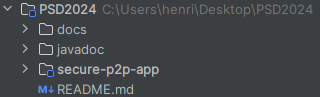
\includegraphics[width=15cm]{image1.png}
    \caption{IDE Project Folders}
\end{figure}
\begin{figure}[htp]
    \centering
    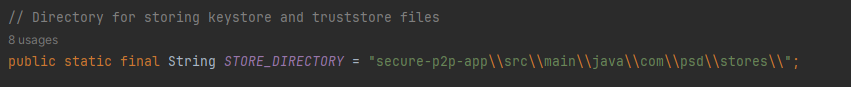
\includegraphics[width=15cm]{image2.png}
    \caption{EncriptionServer.java - STORES relative path}
\end{figure}
\clearpage
\textbf{To run the application, follow these steps:}
\begin{enumerate}
    \item Install Maven
    \item Compile the application if there are changes in the source code.
    \begin{verbatim}
        mvn clean compile -f "C:\Path\To\Your\Project\secure-p2p-app\pom.xml"
    \end{verbatim}
    \item Run \texttt{centralServer}'s main to start the central server.
    \item For each peer (user), run \texttt{SecureP2PMessagingApp}'s main to start the application using this command line:
    \begin{verbatim}
        mvn exec:java -f "C:\Path\To\Your\Project\secure-p2p-app\pom.xml"
    \end{verbatim}
\end{enumerate}



% Conclusion Section
\subsubsection{Conclusion}
The project meets the requirements of a peer-to-peer messaging system, achieving a high degree of decentralization with a central server used solely for aggregating peer information. Leveraging SSL for secure communication, JavaFX for a responsive user interface, and a structured application architecture, this platform enables secure, organized, and direct messaging between users.



\end{document}